% ##QuantumControl
\documentclass[a4paper, english]{scrartcl}
\usepackage[utf8]{inputenc}
\usepackage{amsmath}
\usepackage{amsfonts}
\usepackage{amssymb}
\usepackage{babel}
\usepackage[cm]{fullpage}
\usepackage{float}
\usepackage{graphicx}
\usepackage{helvet}
\usepackage{hyperref}
\usepackage{mathtools}
\usepackage{nicefrac}
\usepackage{tikz}
\usepackage{pgfplots}
\usepackage{placeins}
\usepackage{verbatim}
\usepackage{xcolor}
\definecolor{gr}{gray}{0.9}
\renewcommand{\familydefault}{\sfdefault}
\title{Quantum Control}
\subtitle{Replacement of $H$ with $Y_{90}$}
\author{Ben Criger}
\date{\today}
\input{Qcircuit.tex}
\usepackage{amsmath}
\usepackage{bbold}
\usepackage{color}
\usepackage{stmaryrd}
\usepackage{calc}
\usepackage{verbatim}
\usepackage{mathtools}
\usepackage{xspace}
\DeclarePairedDelimiter{\ceil}{\lceil}{\rceil}
\DeclarePairedDelimiter{\floor}{\lfloor}{\rfloor}
\DeclareMathOperator{\Span}{span}
\usepackage{tikz}
\usetikzlibrary{calc}
\providecommand{\polygon}[2]{%
  let \n{len} = {2*#2*tan(360/(2*#1))} in
 ++(0,-#2) ++(\n{len}/2,0) \foreach \x in {1,...,#1} { -- ++(\x*360/#1:\n{len})}}

\DeclareMathOperator\erf{erf}
\DeclareMathOperator\erfc{erfc}

\newsavebox\CBox
\newcommand\hcancel[2][0.5pt]{%
  \ifmmode\sbox\CBox{$#2$}\else\sbox\CBox{#2}\fi%
  \makebox[0pt][l]{\usebox\CBox}%  
  \rule[0.5\ht\CBox-#1/2]{\wd\CBox}{#1}}

\providecommand{\drv}[1]{\frac{\partial }{\partial #1}}
\providecommand{\drf}[2]{\frac{\partial #1}{\partial #2}}
\providecommand{\ddrf}[3]{\frac{\partial^2 #1}{\partial #2 \partial #3}}
\providecommand{\ddid}[3]{\frac{\partial^2 #1}{\partial #2 \partial #3} = \dfrac{\partial^2 #1}{\partial #3 \partial #2}}

\providecommand{\tr}{\mathrm{tr}}
 
\providecommand{\ket}[1]{\left \vert #1 \right \rangle}
\providecommand{\bra}[1]{\left \langle #1 \right \vert}
\providecommand{\braket}[2]{\left \langle #1 \left \vert #2 \right. \right \rangle}
\providecommand{\angles}[1]{\left \langle #1 \right \rangle}
\providecommand{\elem}[3]{\left \langle #1 \left \vert \vphantom{#1#2#3} #2 \right \vert #3 \right \rangle}
\providecommand{\delem}[2]{\left \langle #1 \left \vert \vphantom{#1#2} #2 \right \vert #1 \right \rangle}
\providecommand{\ketbra}[2]{\ket{#1} \! \bra{#2}}
\providecommand{\proj}[1]{\ketbra{#1}{#1}}
\providecommand{\twonorm}[1]{\| #1 \|_2}
\providecommand{\abs}[1]{\left \vert #1 \right \vert}
\providecommand{\set}[1]{\left \lbrace #1 \right \rbrace}
\providecommand{\group}[1]{\left \langle #1 \right \rangle}
\providecommand{\red}[1]{\textcolor[rgb]{0.5,0,0}{#1}}
\providecommand{\blue}[1]{\textcolor[rgb]{0,0,0.5}{#1}}
\providecommand{\green}[1]{\textcolor[rgb]{0,0.5,0}{#1}}
\providecommand{\conjecture}[1]{\red{#1 (check this).}}
\providecommand{\future}[1]{\green{#1 (do this later).}}
\providecommand{\id}{\hat{\mathbb{1}}}
\providecommand{\com}[2]{\left[#1,\,#2 \right]}
\providecommand{\acom}[2]{\left \lbrace #1,\,#2 \right \rbrace}
\providecommand{\diss}[2]{\mathcal{D}\left[ #1 \right]\left( #2 \right)}
\providecommand{\meas}[2]{\mathcal{M}\left[ #1 \right]\left( #2 \right)}
\providecommand{\lindtwo}[2]{ #1 #2 #1^{\dagger} - \dfrac{1}{2} \left \lbrace #1^{\dagger} #1,\,#2 \right \rbrace }
\providecommand{\lindthree}[3]{ #1 #2 #3 - \dfrac{1}{2} \acom{#3 #1}{#2} }
\providecommand{\lindfour}[4]{ #1 #2 #3 - \dfrac{1}{2} \acom{#4}{#2} }
\providecommand{\meastwo}[2]{ #1 #2 + #2 #1^{\dagger} - \tr \left( #1 #2 + #2 #1^{\dagger} \right) #2 }
\providecommand{\tenscom}[4]{\com{#1\otimes #2}{#3 \otimes #4}=\dfrac{1}{2}\left( \com{#1}{#3} \otimes \acom{#2}{#4} + \acom{#1}{#3} \otimes \com{#2}{#4} \right)}
\providecommand{\tenscomsimple}[4]{\com{#1\otimes #2}{#3 \otimes #4} = #1 #3 \otimes \com{#2}{#4} + \com{#1}{#3} \otimes  #4 #2}
\providecommand{\tensacom}[4]{\acom{#1\otimes #2}{#3 \otimes #4}=\dfrac{1}{2}\left( \com{#1}{#3} \otimes \com{#2}{#4} + \acom{#1}{#3} \otimes \acom{#2}{#4} \right)}
\providecommand{\trace}[1]{\mathrm{tr} \left( #1 \right)}
\providecommand{\comp}{\mathop{\bigcirc}}
\providecommand{\swap}{\textsc{swap}\xspace}
\providecommand{\cnot}{\textsc{cnot}\xspace}
\providecommand{\cz}{\textsc{cz}\xspace}
\providecommand{\col}{\textrm{col}}
\providecommand{\qec}[3]{\llbracket #1,\,#2,\,#3 \rrbracket}
\providecommand{\set}[1]{\left \lbrace #1 \right \rbrace}
\renewcommand{\Im}{\textrm{Im}}
\renewcommand{\Re}{\textrm{Re}}
\providecommand{\lind}{\mathcal{L}}
%\providecommand{\norm}[2]{\left \vert \left \vert #2 \right \vert \right \vert_{#1}}
\providecommand{\supp}[1]{\mathrm{supp}\left( #1 \right)}
\providecommand{\given}{\, \middle \vert \,}
\providecommand{\suchthat}{\, \middle \vert \,}
\providecommand{\diag}[1]{\mathrm{diag}\left( #1 \right)}
\providecommand{\ct}{^{\dagger}}

\providecommand{\norm}[1]{\left \Vert #1 \right \Vert} %only works with amsmath

\providecommand{\ncrit}{$n_{\textrm{crit}}$\xspace}

\renewcommand{\th}{\textrm{th}}
\newcommand{\prob}[1]{p\left(#1 \right)}
\newcommand{\cprob}[2]{p\left(#1\,\left\vert\vphantom{#1#2}\right. #2\right)}

\makeatletter
\providecommand{\pr}[2]{p\left(#1\,\middle|\,#2\right)}
\newcommand{\pushright}[1]{\ifmeasuring@#1\else\omit\hfill$\displaystyle#1$\fi\ignorespaces}
\newcommand{\pushleft}[1]{\ifmeasuring@#1\else\omit$\displaystyle#1$\hfill\fi\ignorespaces}
\makeatother
\newlength\figureheight
\newlength\figurewidth
\setlength\figureheight{7cm}
\setlength\figurewidth{12cm}

\providecommand{\cnot}{\textsc{cnot}}

\usetikzlibrary{decorations.pathreplacing, decorations.pathmorphing, shapes.geometric, calc}

\begin{document}
\maketitle
\section{Introduction}
Theorists and experimentalists like to use different gate sets when designing fault-tolerant protocols, leading to much consternation. 
Theorists like to use the Hadamard gate,
\begin{equation}
H \triangleq \dfrac{1}{\sqrt{2}}\begin{bmatrix}
1 & 1 \\ 1 & -1
\end{bmatrix},
\end{equation}
because its action on the Pauli operators under conjugation can be written without adding any minus signs:
\begin{flalign}
HXH^{\dagger} &= Z \\
HZH^{\dagger} &= X \\
HYH^{\dagger} &= Y. 
\end{flalign}
No minus signs, no problem. 
Experimentalists, on the other hand, like to rotate their qubit states around cardinal axes of the Bloch sphere.  We focus on the $Y_{\pm 90}$ gates,
\begin{equation}
Y_{\pm 90} = \begin{bmatrix}
\cos \left( \pm \nicefrac{\pi}{4} \right) & -\sin \left( \pm \nicefrac{\pi}{4} \right) \\
\sin \left( \pm \nicefrac{\pi}{4} \right) & \cos \left( \pm \nicefrac{\pi}{4} \right)
\end{bmatrix} = \dfrac{1}{\sqrt{2}} \begin{bmatrix}
1 & \mp 1 \\ \pm 1 & 1
\end{bmatrix},
\end{equation}
which are often used as replacements for the Hadamard in experimental implementations.

The remainder of this document contains a few facts about this replacement
\section{Effect on Basis States}
\begin{flalign}
H\ket{0} = \ket{+} &= Y_{90} \ket{0} \\
H\ket{1} = \ket{-} &= -Y_{90} \ket{1}
\end{flalign}
Up to an irrelevant global phase, the effects of Hadamard and $Y_{90}$ on computational basis states are identical.
\section{Matrix Identities}
\begin{flalign}
Y_{90} Z &= \dfrac{1}{\sqrt{2}} \begin{bmatrix}
1 & -1 \\  1 & 1
\end{bmatrix}\begin{bmatrix}
1 & 0 \\ 0 & -1
\end{bmatrix} = \dfrac{1}{\sqrt{2}} \begin{bmatrix}
1 & 1 \\  1 & -1
\end{bmatrix} = H  \\
Z Y_{-90} &= \dfrac{1}{\sqrt{2}} \begin{bmatrix}
1 & 0 \\ 0 & -1
\end{bmatrix}\begin{bmatrix}
1 & 1 \\ -1 & 1
\end{bmatrix} = \dfrac{1}{\sqrt{2}} \begin{bmatrix}
1 & 1 \\  1 & -1
\end{bmatrix} = H 
\end{flalign}
A Hadamard in a theorist's circuit can be decomposed into $Y_{\pm 90}$ and Pauli $Z$ operations, and we get to choose where to put the $Z$ by selecting the $\pm$ sign. 
The typical goal is to produce $Z$s that cancel with one another, so that the need not actually be performed in an experiment. 
We give an example of this in the next section.
\section{Circuit Identities}
Consider the decomposition of a \cnot into two $H$s and a \textsc{cphase}:
\begin{figure}[!ht]
\centering
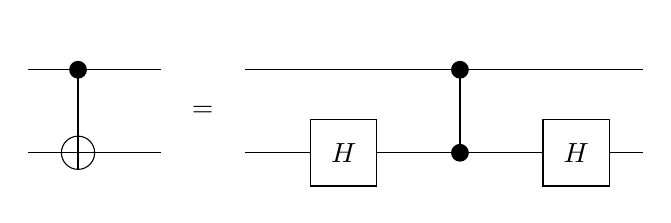
\begin{tikzpicture}[scale=2.000000,x=1pt,y=1pt]
\filldraw[color=white] (0.000000, -7.500000) rectangle (111.000000, 22.500000);
% Drawing wires
% Line 1: a W
\draw[color=black] (0.000000,15.000000) -- (111.000000,15.000000);
% Line 2: b W
\draw[color=black] (0.000000,0.000000) -- (111.000000,0.000000);
% Done with wires; drawing gates
% Line 4: +b a
\draw (9.000000,15.000000) -- (9.000000,0.000000);
\begin{scope}
\draw[fill=white] (9.000000, 0.000000) circle(3.000000pt);
\clip (9.000000, 0.000000) circle(3.000000pt);
\draw (6.000000, 0.000000) -- (12.000000, 0.000000);
\draw (9.000000, -3.000000) -- (9.000000, 3.000000);
\end{scope}
\filldraw (9.000000, 15.000000) circle(1.500000pt);
% Line 5: =
\draw[fill=white,color=white] (24.000000, -6.000000) rectangle (39.000000, 21.000000);
\draw (31.500000, 7.500000) node {$=$};
% Line 6: b H
\begin{scope}
\draw[fill=white] (57.000000, -0.000000) +(-45.000000:8.485281pt and 8.485281pt) -- +(45.000000:8.485281pt and 8.485281pt) -- +(135.000000:8.485281pt and 8.485281pt) -- +(225.000000:8.485281pt and 8.485281pt) -- cycle;
\clip (57.000000, -0.000000) +(-45.000000:8.485281pt and 8.485281pt) -- +(45.000000:8.485281pt and 8.485281pt) -- +(135.000000:8.485281pt and 8.485281pt) -- +(225.000000:8.485281pt and 8.485281pt) -- cycle;
\draw (57.000000, -0.000000) node {$H$};
\end{scope}
% Line 7: a b
\draw (78.000000,15.000000) -- (78.000000,0.000000);
\filldraw (78.000000, 15.000000) circle(1.500000pt);
\filldraw (78.000000, 0.000000) circle(1.500000pt);
% Line 8: b H
\begin{scope}
\draw[fill=white] (99.000000, -0.000000) +(-45.000000:8.485281pt and 8.485281pt) -- +(45.000000:8.485281pt and 8.485281pt) -- +(135.000000:8.485281pt and 8.485281pt) -- +(225.000000:8.485281pt and 8.485281pt) -- cycle;
\clip (99.000000, -0.000000) +(-45.000000:8.485281pt and 8.485281pt) -- +(45.000000:8.485281pt and 8.485281pt) -- +(135.000000:8.485281pt and 8.485281pt) -- +(225.000000:8.485281pt and 8.485281pt) -- cycle;
\draw (99.000000, -0.000000) node {$H$};
\end{scope}
% Done with gates; drawing ending labels
% Done with ending labels; drawing cut lines and comments
% Done with comments
\end{tikzpicture}
\caption{Decomposition of the theorist's \cnot into an experimentalist's \textsc{cphase} and some $H$s. Noting that $H$ is hermitian (another nice feature for theorists), this follows from the fact that $HZH=X$.}
\end{figure}

We know that $Z$ commutes with \textsc{cphase} (since the matrices for these gates in the computational basis are both diagonal), so that the Pauli $Z$s which result from decomposing the $H$s can be made to cancel:
\begin{figure}[!ht]
\centering
\input{HY90CircuitIdentity.tikz}
\caption{A \cnot expressed using only experimentalist's gates.
Note that other gate sets may be available in any given implementation of quantum computing.
Note also that this identity applies to all imput states, not just computational basis states.
Note, thirdly, that the order of gates in a circuit is the reverse of the order of matrices in a product. }
\end{figure}
\end{document}